\subsection{Elastic selection} 
\label{sec:elastic_selection}
The $e P \,\rightarrow\, e' \,P'\,$ elastic reaction is useful for many purposes. 
The constraint allows one to determine systematic errors and corrections,
on one or more variables.
The hadronic mass of the $P\, \pi^0$ system is close to $M_P$, so 
one can assume that those corrections hold for the $\Delta(1232)$ kinematics as well
as they do for the elastic kinematics.

The Bethe Heitler (B.H.) process $eP\rightarrow eP\gamma$ discussed in \ref{sec:bethe}
is included in elastic $eP$ events, and cuts are determined to select
only low energy (soft) photons.

I present here a series of cuts for e1-6 data to achieve exclusive 
elastic selection after electron and proton particle ID.

\hfill\\

{\bf\boldmath $W$ cut}

The first cut, illustrated in \F{fig:elastic_cuts_s2} a),  is on $W$, the outgoing hadron mass, which for elastic scattering
is the mass of the proton. 
A gaussian is fitted to the $W$ distribution for each sector and 3 $\sigma$ around the mean
determine the $W$ cut. 

\hfill\\

{\bf\boldmath $M_x(eP)$ cut}

The second cut is on the missing mass of the outgoing $e\,P$ system. See \F{fig:elastic_cuts_s2} b). 
No particles except B.H. photons are produced during elastic scattering, 
therefore the missing mass must be zero.
A gaussian is fitted to the $M_x(P)$ distribution for each sector and 3 $\sigma$ around the mean
represents the $M_x(EP)$ cut.

\hfill\\

{\bf\boldmath $\Delta \theta$ cut}


The elastic constraint allows us to determine the proton angle in the lab $\theta^P_{calc}$
using only the outgoing electron angle and energy.
Assuming that the scattered electron doesn't change direction when it emits a photon (peaking approximation),
this calculation is independent of the outgoing electron energy and therefore it is independent of
 post-radiative effects shown on \F{fig:prepost} b). \\
The third cut is on $\Delta\theta = \theta^P_{meas} - \theta^P_{calc}$ (\F{fig:elastic_cuts_s2} c) where
$$
 \tan\theta^P_{calc} =  \Dfrac{1}{(1+\Dfrac{E}{M_P})\tan\Dfrac{\theta_{e'}}{2}}
$$
A gaussian is fitted to the $\Delta\theta$ distribution for each sector and 2 $\sigma$ around the mean
represents the $\Delta\theta$ cut.

\hfill\\


\begin{figure}
 \begin{center}
 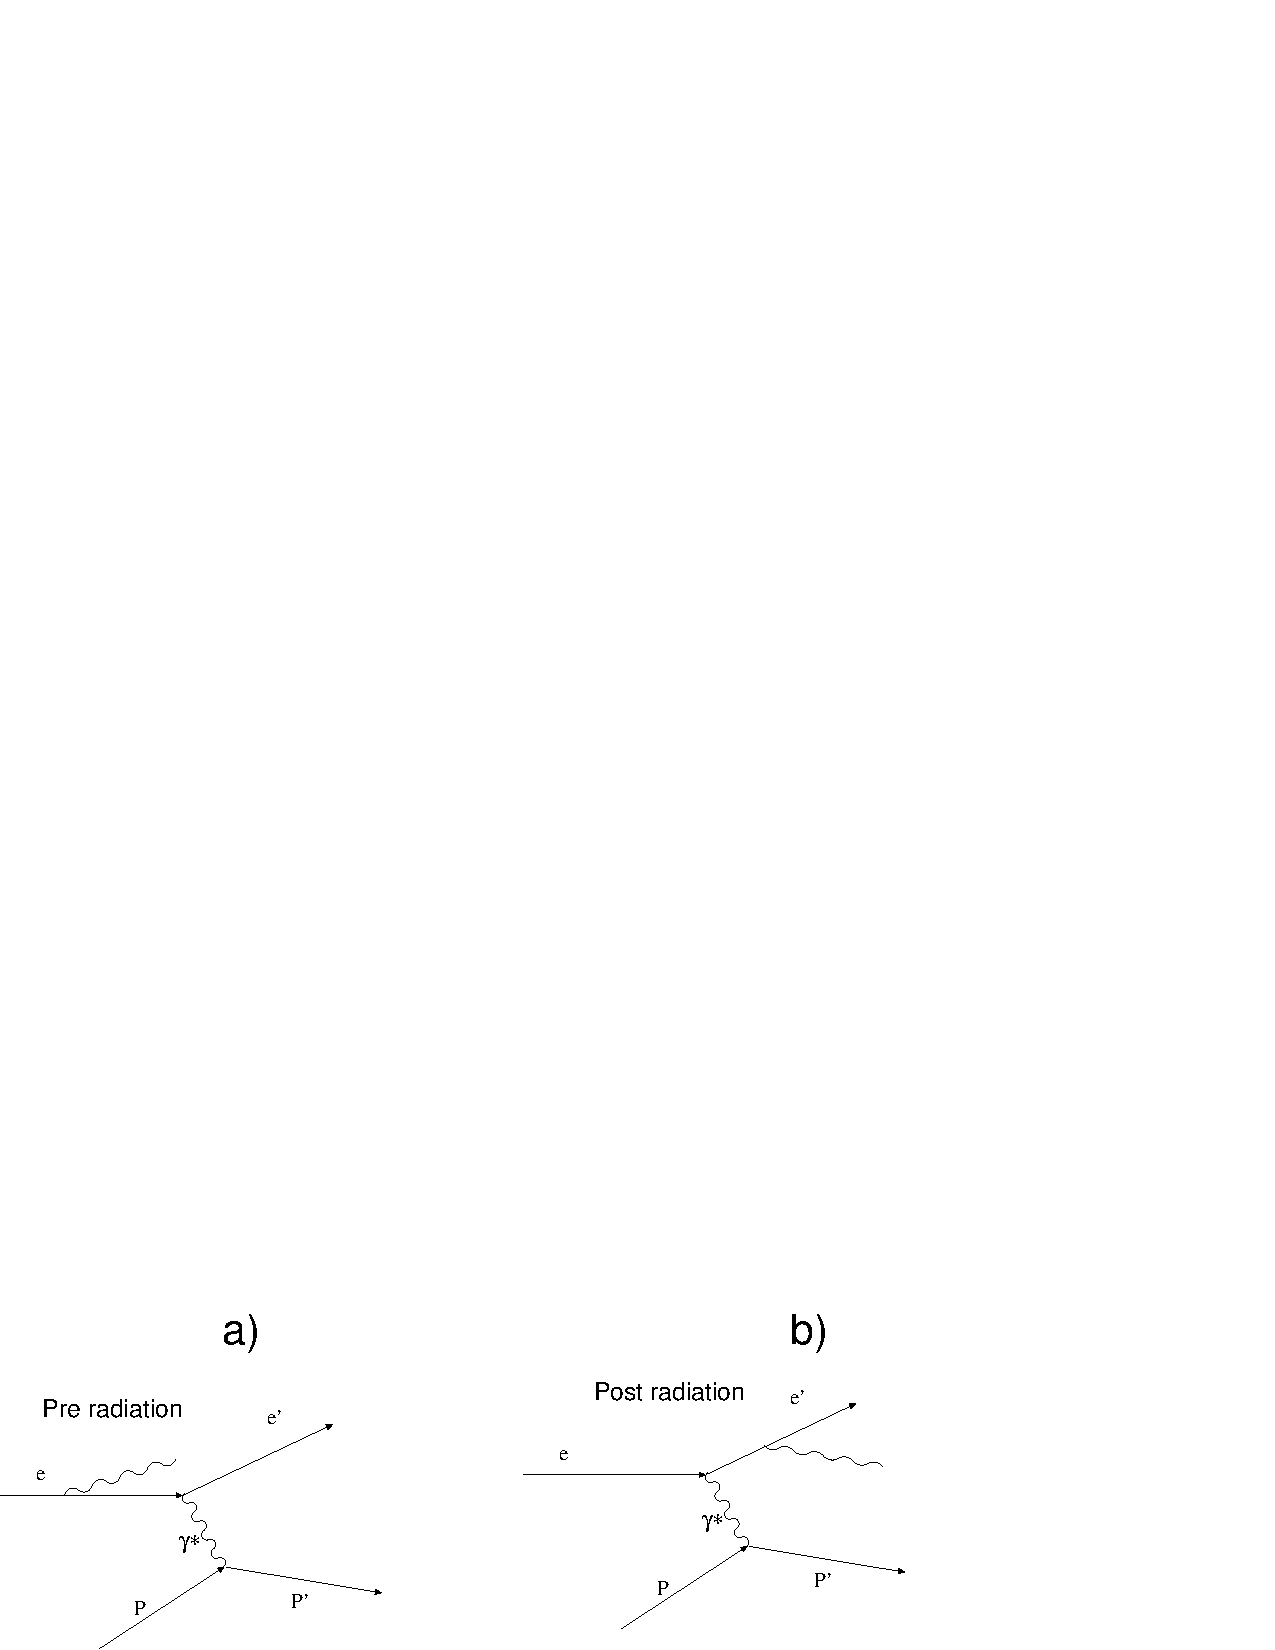
\includegraphics[width = 13cm, bb=-60 -20 450 300]{data_reduction/kine_corr/img/prepostradiation} 
 \caption[Radiative elastic events]
         { Radiative elastic events. a) pre-radiation. A photon is emitted by the incoming electron.
                    b) post-radiation. A photon is emitted by the outgoing electron. }
 \label{fig:prepost}
 \end{center}
\end{figure}


{\bf\boldmath$\Delta \theta_2$ cut\\}
\vspace{-0.8 cm}

The elastic constraint allow us to determine the proton angle in the lab $\theta^P_{calc2}$
using only the incident electron energy and the outgoing electron angle.
This calculation is independent of the incident electron energy and therefore it is independent of
pre-radiative effects shown on the \F{fig:prepost} a).

The fourth cut is on $\Delta\theta_2 = \theta^P_{meas} - \theta^P_{calc2}$ (\F{fig:elastic_cuts_s2} d) where
$$
 \tan\theta^P_{calc2} =  \Dfrac{1}{(1+\Dfrac{E'}{M_P-E'+E'\cos\theta_{e'}})\tan\Dfrac{\theta_{e'}}{2}}
$$
A gaussian is fitted to the $\Delta\theta_2$ distribution for each sector and 2 $\sigma$ around the mean
represents the $\Delta\theta_2$ cut.

\hfill\\

{\bf\boldmath$\Delta\phi$ cut} \\
The fifth and final cut is on the difference between the electron and proton 
azimuthal angle  $\Delta\phi$ (\F{fig:elastic_cuts_s2} e).
Both electrons and protons, in the peaking approximation and for elastic events,  
lie in the same plane therefore $\Delta\phi$ must be equal to $\pi$.

A gaussian is fitted to the $\Delta\phi$ distribution for each sector and two $\sigma$s around the mean
represents the $\Delta\phi$ cut.


\begin{figure}[h]
 \begin{center}
 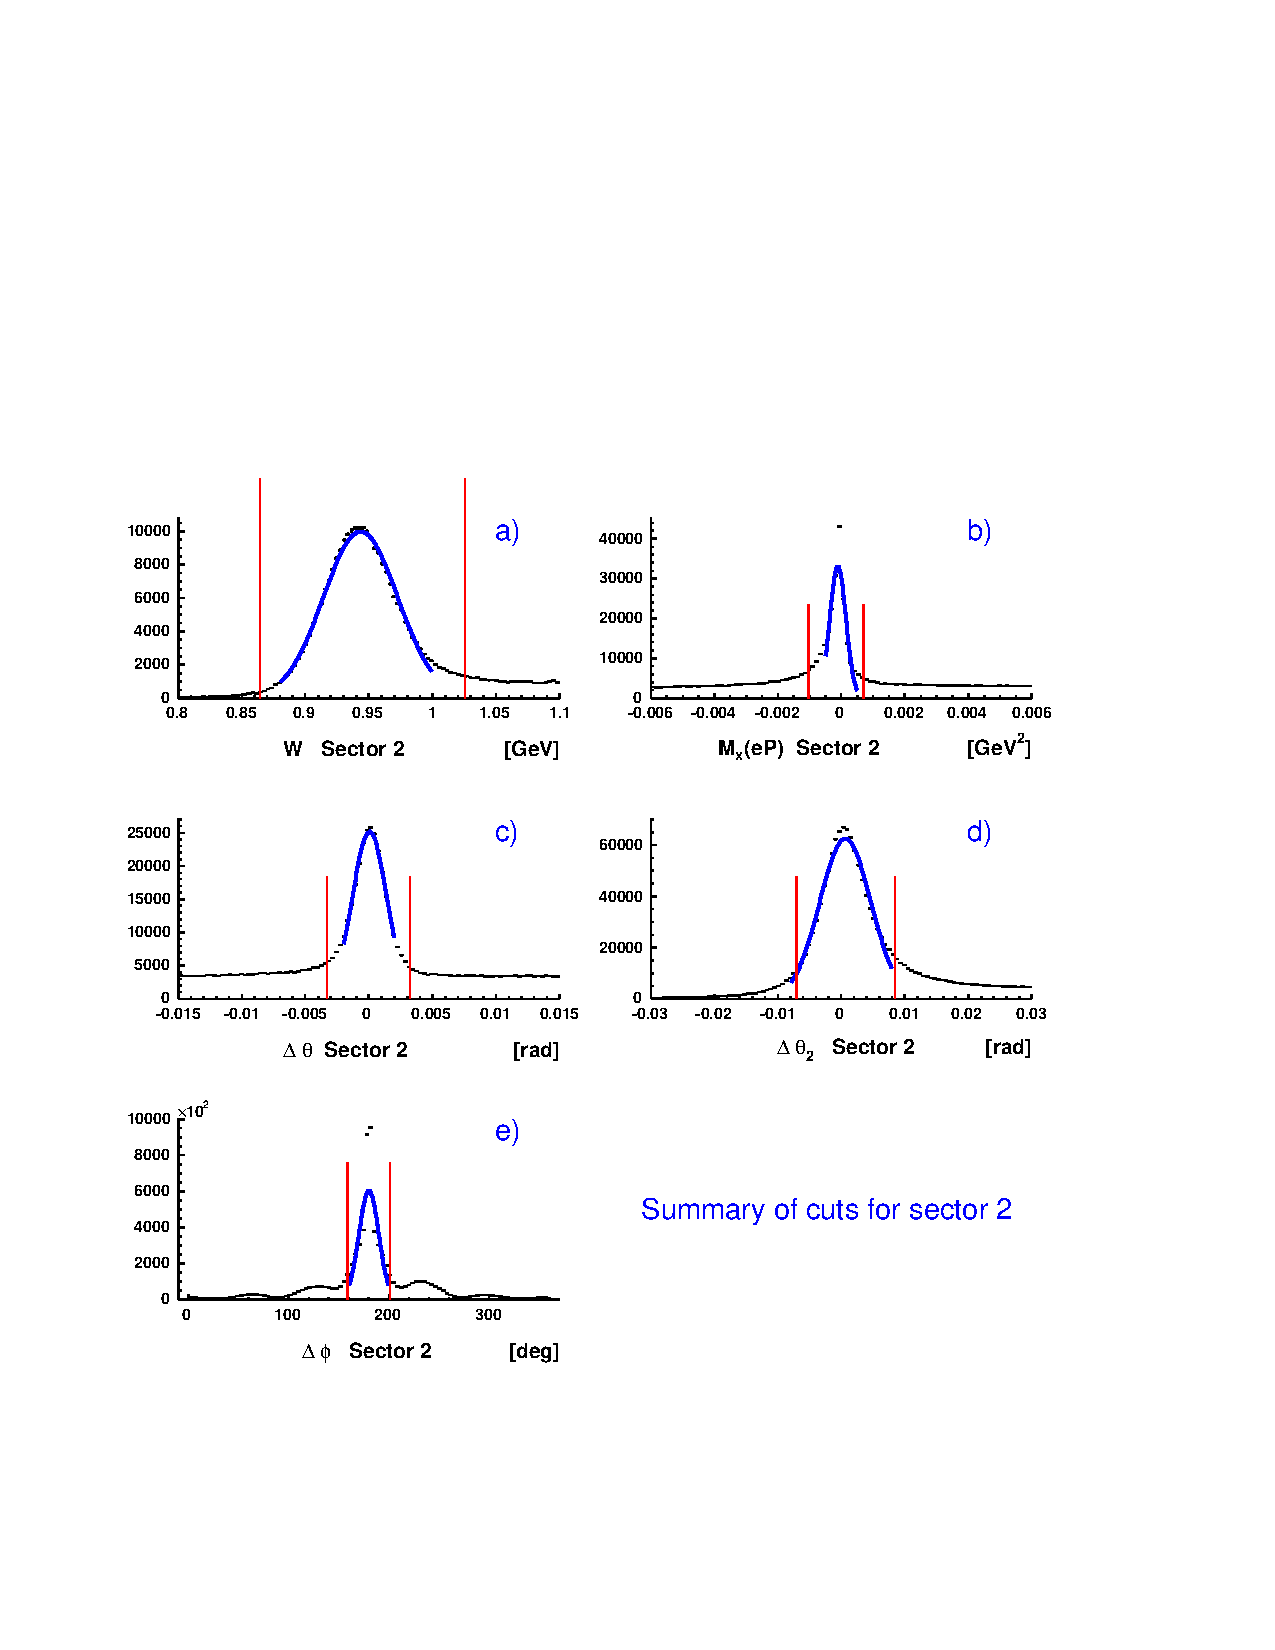
\includegraphics[width = 12cm, bb=60 130 540 590]{data_reduction/kine_corr/img/elastic_cuts_s2} 
  \caption[The cuts for elastic selection for sector 2]
          { The cuts for elastic selection for sector 2. (a) W mass cut. (b) Missing $(eP)$ mass cut.
	             (c) $\Delta\theta$ cut. (d) $\Delta\theta_2$ cut. (e) Coplanarity cut. }
 \label{fig:elastic_cuts_s2}
 \end{center}
\end{figure}






